% !TEX encoding = UTF-8 Unicode
% Thesis defense slides: 20 main slides, followed by backup slides for technical questions.

\documentclass[aspectratio=169,11pt]{beamer}

\usepackage[greek,english]{babel}
\usepackage{alphabeta}
\usepackage{booktabs}
\usepackage{tabularx}

\usetheme[progressbar=frametitle,numbering=counter,block=fill]{metropolis}
\setbeamertemplate{frame footer}{Ilya Saunkin \textendash{} Categorizing citations in scientific publications}

\graphicspath{{../tex/include/}}

% Inline screenshot of a UI control, as in the thesis
\newcommand{\uicontrol}[1]{\raisebox{-.3\height}{\includegraphics[scale=.12]{ui/#1}}}

\title{Categorizing citations in scientific publications}
\subtitle{Κατηγοριοποίηση αναφορών σε επιστημονικές δημοσιεύσεις}
\author{Ilya Saunkin}
\institute{%
  Department of Informatics and Telecommunications, University of Peloponnese\\[1ex]
  \footnotesize Supervisor: Spiros Skiadopoulos\quad Committee: Costas Vassilakis%
}
\date{November 2026}
\titlegraphic{\hfill
\includegraphics[height=1.6cm]{logo-uop}}

\begin{document}

% 1
\maketitle

% 2
\begin{frame}{Outline}
  \begin{enumerate}
    \item Motivation and problem statement
    \item Self-citations: one citation, different answers
    \item Data sources
    \item Methodology: data model and classification
    \item The system
    \item Evaluation
    \item Conclusions and future work
  \end{enumerate}
\end{frame}

% 3
\begin{frame}{Citations and self-citations}
  \begin{itemize}
    \item If a publication $c$ refers to a publication $p$, we say that $c$ \alert{cites} $p$
    \item Citation counts are aggregated per author to estimate the influence of a researcher
    \item Not all citations carry the same meaning:
      \begin{itemize}
        \item \alert{self-citation}: at least one author appears in both publications
        \item \alert{external citation}: no overlap between the authors
      \end{itemize}
    \item Self-citations occur naturally in cumulative research
    \item Used excessively, they inflate citation-based metrics
  \end{itemize}
\end{frame}

% 4
\begin{frame}{Problem statement}
  Given a specific author $A$, we want to:
  \begin{enumerate}
    \item identify the publications of $A$
    \item compute the total number of citations received by these publications
    \item distinguish between self-citations and external citations
  \end{enumerate}
  \vspace{1em}
  The most important step is the third one: the classification of citations, based on author overlap.
\end{frame}

% 5
\begin{frame}{Example: two articles}
  \small
  \begin{tabularx}{\textwidth}{@{}lX@{}}
    \toprule
    {[GPK2007]} & Gabriel Ghinita, Panos Kalnis, Spiros Skiadopoulos:
      \emph{PRIVE: anonymous location-based queries in distributed mobile systems}. WWW 2007 \\
    {[KGMP2007]} & Panos Kalnis, Gabriel Ghinita, Kyriakos Mouratidis, Dimitris Papadias:
      \emph{Preventing Location-Based Identity Inference in Anonymous Spatial Queries}. IEEE TKDE 2007 \\
    \bottomrule
  \end{tabularx}
  \vspace{1em}
  \normalsize
  \begin{itemize}
    \item [KGMP2007] cites [GPK2007]
    \item Ghinita and Kalnis appear in \alert{both} articles
    \item Skiadopoulos appears \alert{only} in the cited article
  \end{itemize}
\end{frame}

% 6
\begin{frame}{One citation, different answers}
  \begin{columns}[T]
    \begin{column}{.55\textwidth}
      \begin{itemize}
        \item For Kalnis and Ghinita: a \alert{self-citation}
        \item For Skiadopoulos, it depends on the approach:
          \begin{itemize}
            \item compare the authors of both papers: self-citation
            \item consider only the authors of the citing paper: external citation
          \end{itemize}
        \item Definitions vary across studies
        \item Platforms such as Scopus filter out self-citations, but do not always explain how
      \end{itemize}
    \end{column}
    \begin{column}{.42\textwidth}
      \centering
      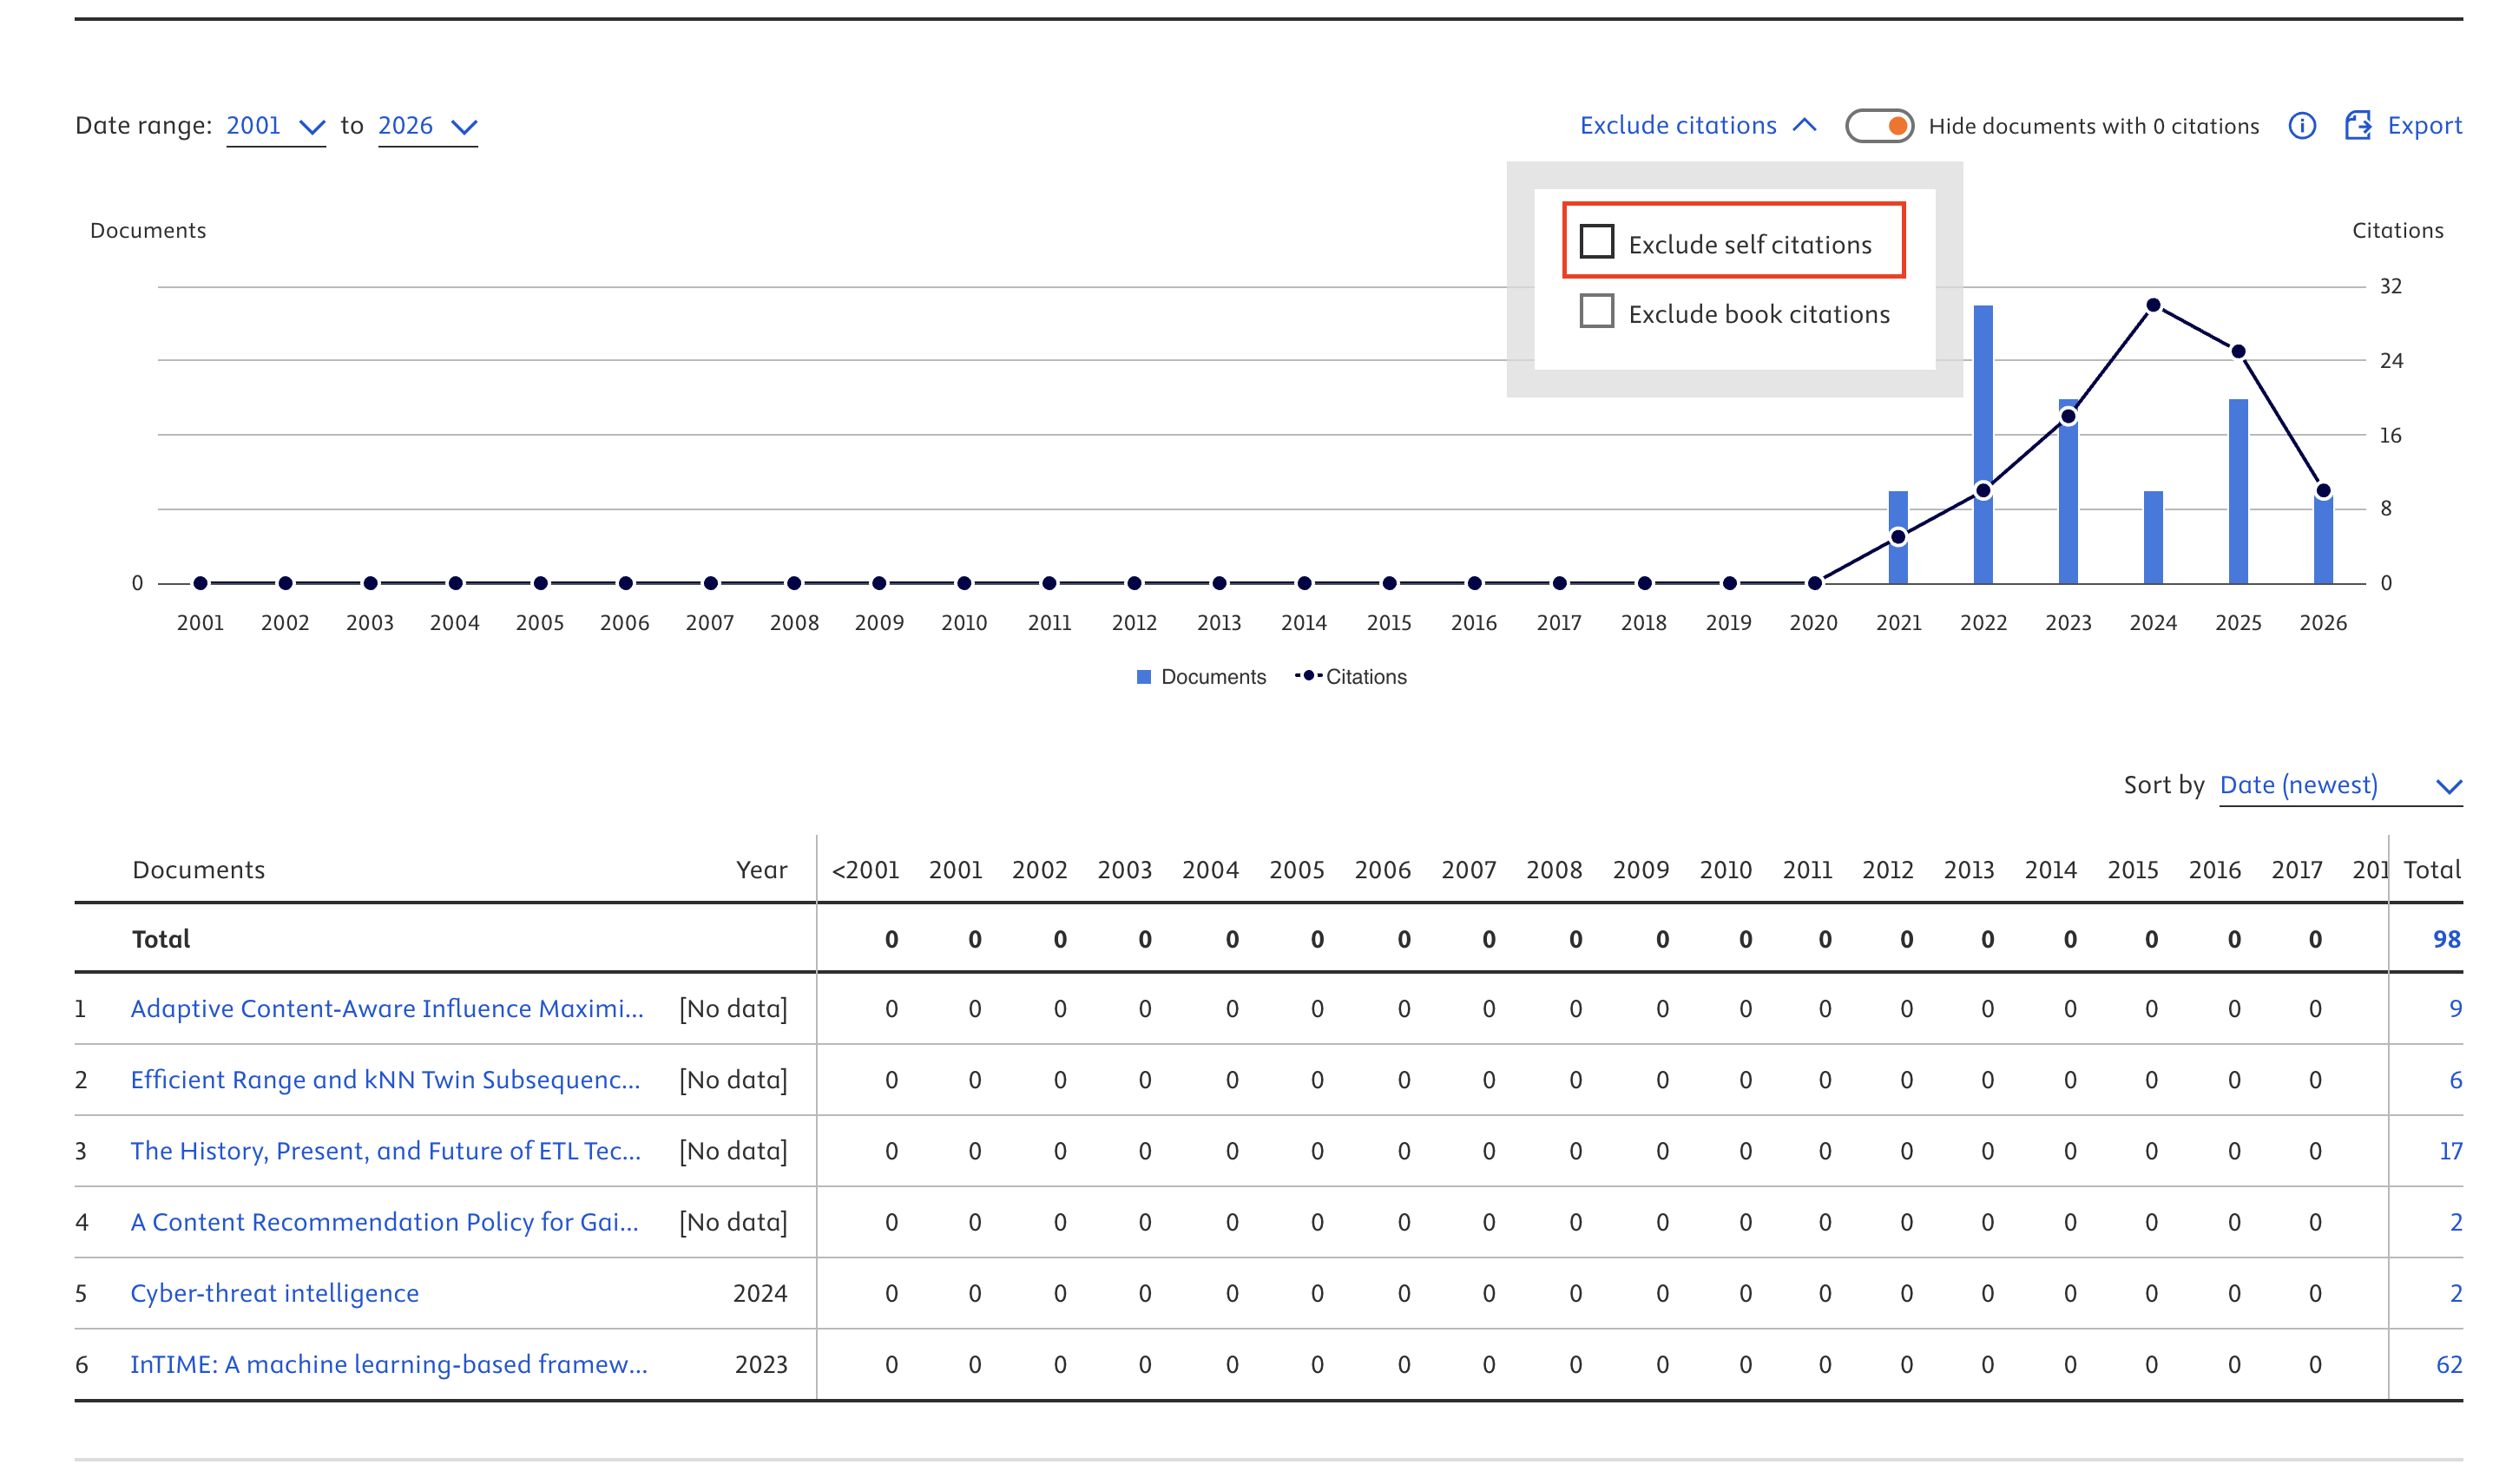
\includegraphics[width=\textwidth]{fig-scopus-2}\\
      \scriptsize Scopus: excluding self-citations
    \end{column}
  \end{columns}
\end{frame}

% 7
\begin{frame}{Data sources}
  \scriptsize
  \begin{tabularx}{\textwidth}{@{}lXXll@{}}
    \toprule
    Source & Access & Coverage & Citations & Author data \\
    \midrule
    Google Scholar & No public API; HTML scraping & Largest; all disciplines & Yes & Profile ID; names as text \\
    OpenAlex & Open API, free key & About 271M works & Yes & Author IDs \\
    Semantic Scholar & Open API, free key & Over 200M papers & Yes & Author IDs \\
    CrossRef & Open API, free & Over 180M DOI records & Count only & No author IDs \\
    OpenCitations & Open API and dumps & Over 2B citation links & Yes & ORCID only \\
    DBLP & Open API and dump & 6.6M works; CS only & No & Strong disambiguation \\
    Scopus & Paid subscription & About 90M records & Yes & Scopus author IDs \\
    LLM & Model query & Broad, unverifiable & Yes & No identifiers \\
    \bottomrule
  \end{tabularx}
  \vspace{1ex}

  \normalsize
  Common issues: rate limits, paywalls, inconsistent metadata, no shared author identifiers.
\end{frame}

% 8
\begin{frame}{Selected providers}
  \begin{columns}[T]
    \begin{column}{.48\textwidth}
      \textbf{Implemented}
      \begin{itemize}
        \item \alert{OpenAlex}: open, author IDs, citing works with authors
        \item \alert{Semantic Scholar}: open, author IDs; one request per second
        \item \alert{Google Scholar} via SerpApi: widest coverage; paid per request, names as text
      \end{itemize}
    \end{column}
    \begin{column}{.48\textwidth}
      \textbf{Not implemented}
      \begin{itemize}
        \item CrossRef: no list of citing papers
        \item OpenCitations: no search by author name
        \item DBLP: computer science only, no citations
        \item Scopus: paid subscription
      \end{itemize}
    \end{column}
  \end{columns}
  \vspace{1em}
  Profiles are kept separate per provider: no shared author identifiers.
\end{frame}

% 9
\begin{frame}{Data model}
  \begin{columns}[c]
    \begin{column}{.5\textwidth}
      \begin{itemize}
        \item Entities: \alert{author}, \alert{publication}
        \item Relationships:
          \begin{itemize}
            \item \alert{contribution}: authors write publications (many-to-many)
            \item \alert{citation}: publications cite publications (many-to-many)
          \end{itemize}
        \item The minimum structure needed to classify citations
      \end{itemize}
    \end{column}
    \begin{column}{.48\textwidth}
      \centering
      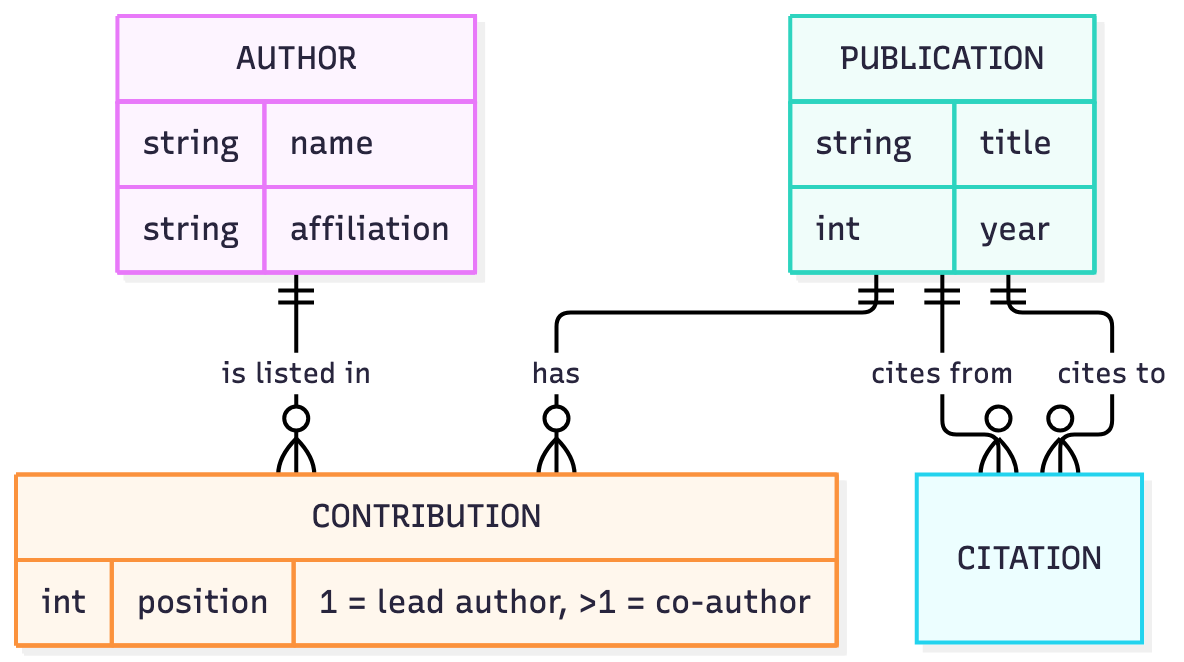
\includegraphics[width=\textwidth]{fig-data-model-er-diagram}
    \end{column}
  \end{columns}
\end{frame}

% 10
\begin{frame}{Classification of citations}
  For any author $A$, a citation $c_j$ of their publication $p_i$ is classified as one of the following:
  \begin{description}
    \item[Direct self-citation] $A$ is also an author of $c_j$
    \item[Co-author self-citation] $A$ is not an author of $c_j$, but $p_i$ and $c_j$ share at least one author
    \item[External citation] no overlap between the authors of $p_i$ and $c_j$
  \end{description}
  \vspace{1ex}
  \begin{itemize}
    \item The example: \alert{direct} for Kalnis and Ghinita, \alert{co-author} for Skiadopoulos
    \item We keep the different views apart, instead of choosing one
  \end{itemize}
\end{frame}

% 11
\begin{frame}{From classification to metrics}
  \begin{columns}[T]
    \begin{column}{.48\textwidth}
      \textbf{Process}
      \begin{enumerate}
        \item Identify all publications $p_i$ of $A$
        \item Collect all incoming citations $c_j$ of each $p_i$
        \item Classify each citation
      \end{enumerate}
    \end{column}
    \begin{column}{.48\textwidth}
      \textbf{Counts for $A$}
      \begin{itemize}
        \item Total number of citations
        \item Self-citations
        \begin{itemize}
          \item direct
          \item co-author
        \end{itemize}
        \item External citations
      \end{itemize}
    \end{column}
  \end{columns}
  \vspace{1em}
  Limitations: rate-limited access, inconsistent coverage, ambiguous author identities.
\end{frame}

% 12
\begin{frame}{System architecture}
  \begin{columns}[c]
    \begin{column}{.45\textwidth}
      \begin{itemize}
        \item Model-View-Controller
        \item Frontend: React single-page application
        \item Backend: Node.js API
          \begin{itemize}
            \item controllers, services, repositories
            \item one connector per provider
          \end{itemize}
        \item SQLite database and response cache
      \end{itemize}
    \end{column}
    \begin{column}{.53\textwidth}
      \centering
      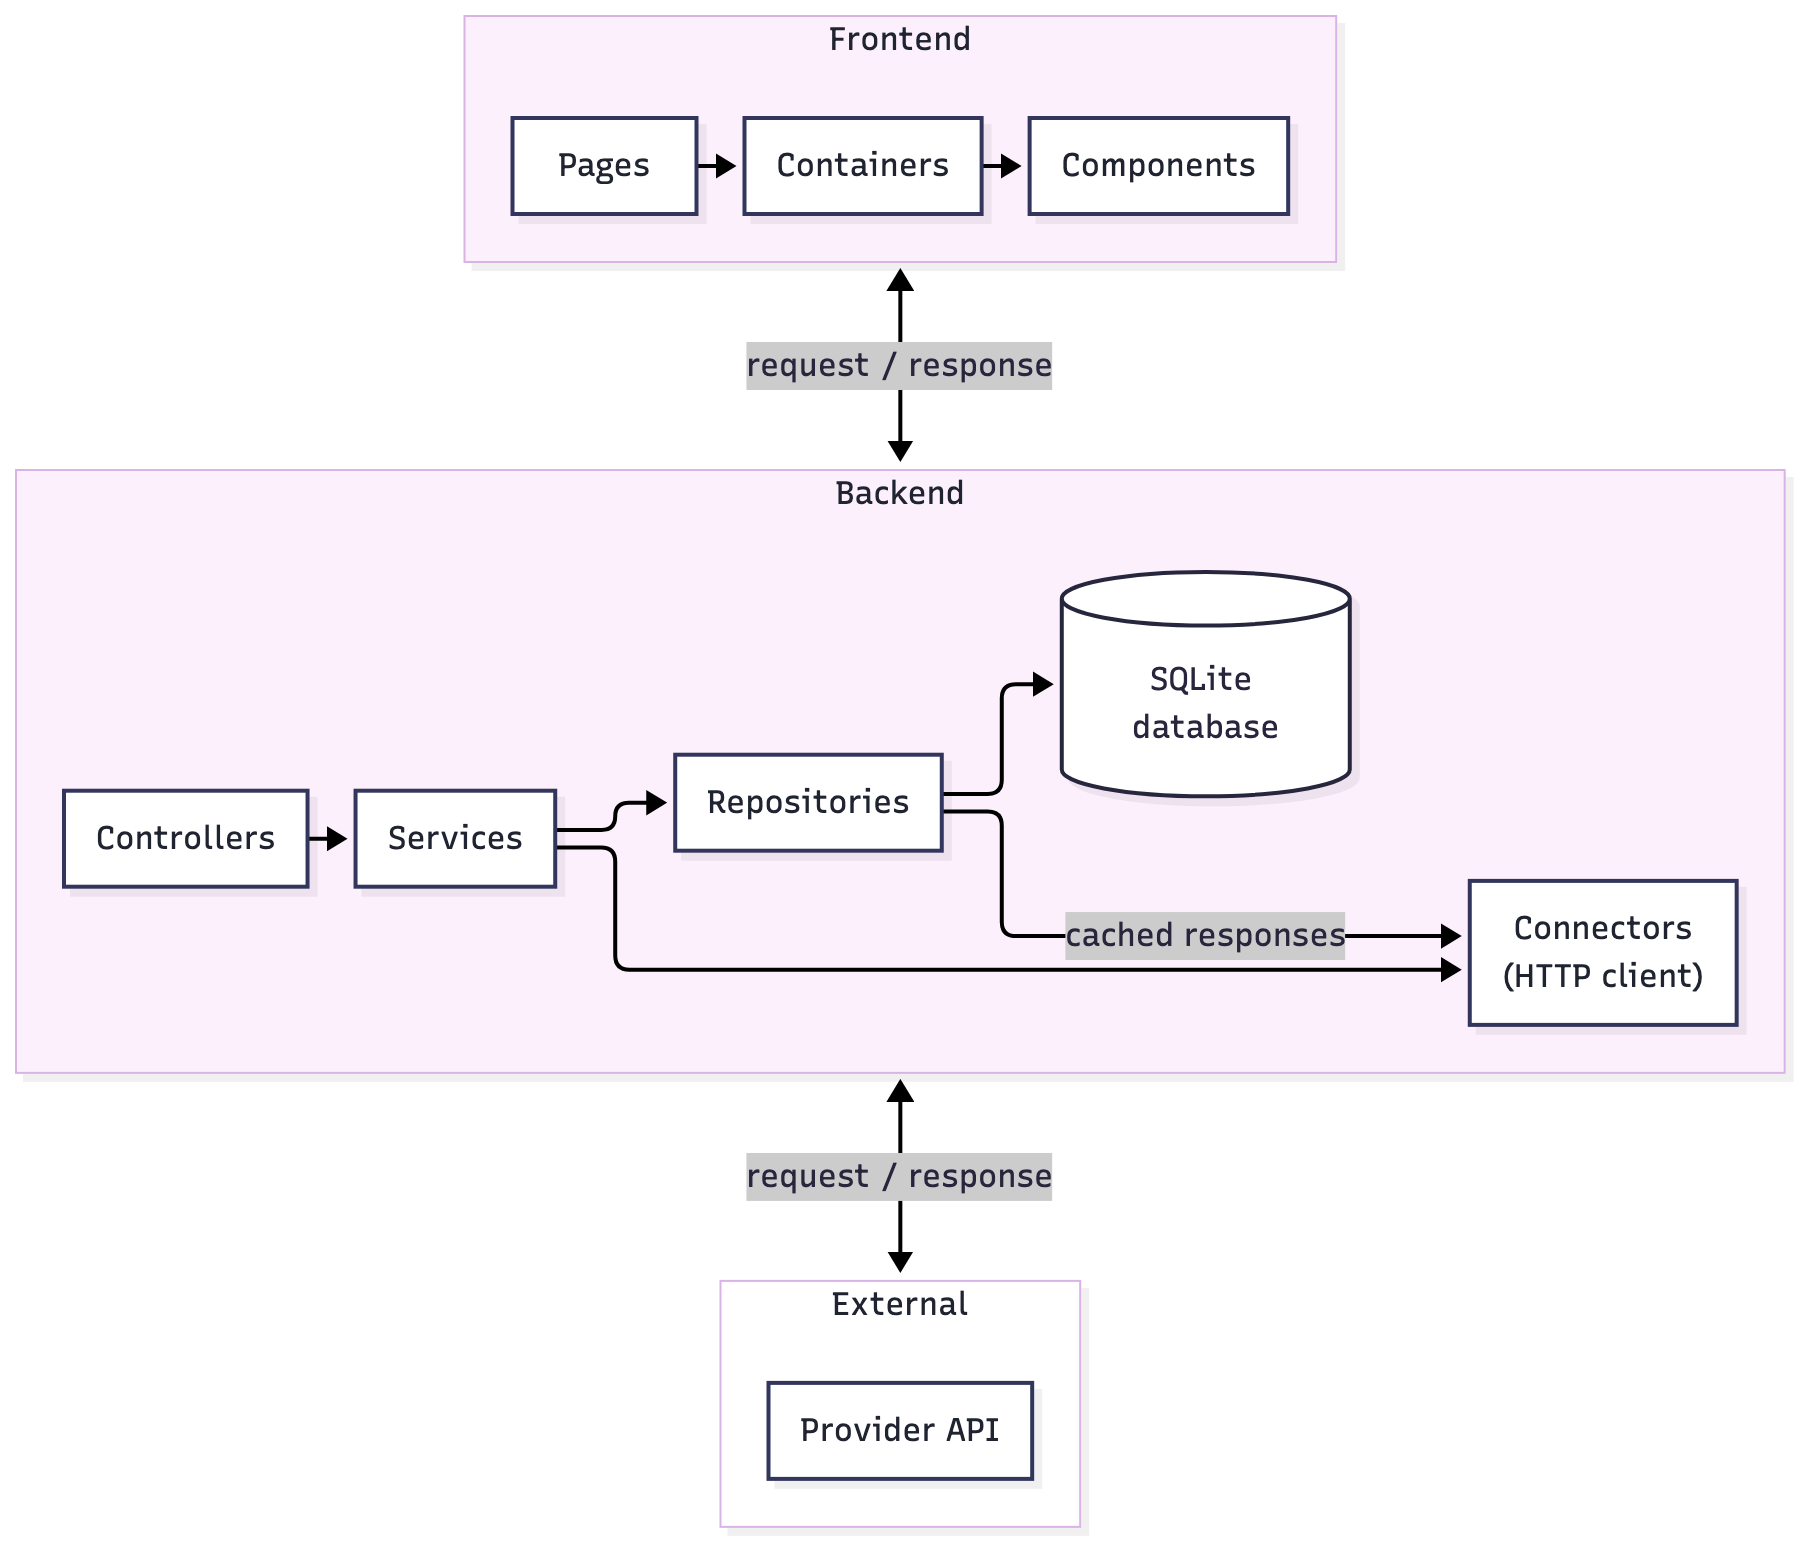
\includegraphics[height=.75\textheight]{fig-arch-mvc-diagram}
    \end{column}
  \end{columns}
\end{frame}

% 13
\begin{frame}{Building the citation graph}
  \centering
  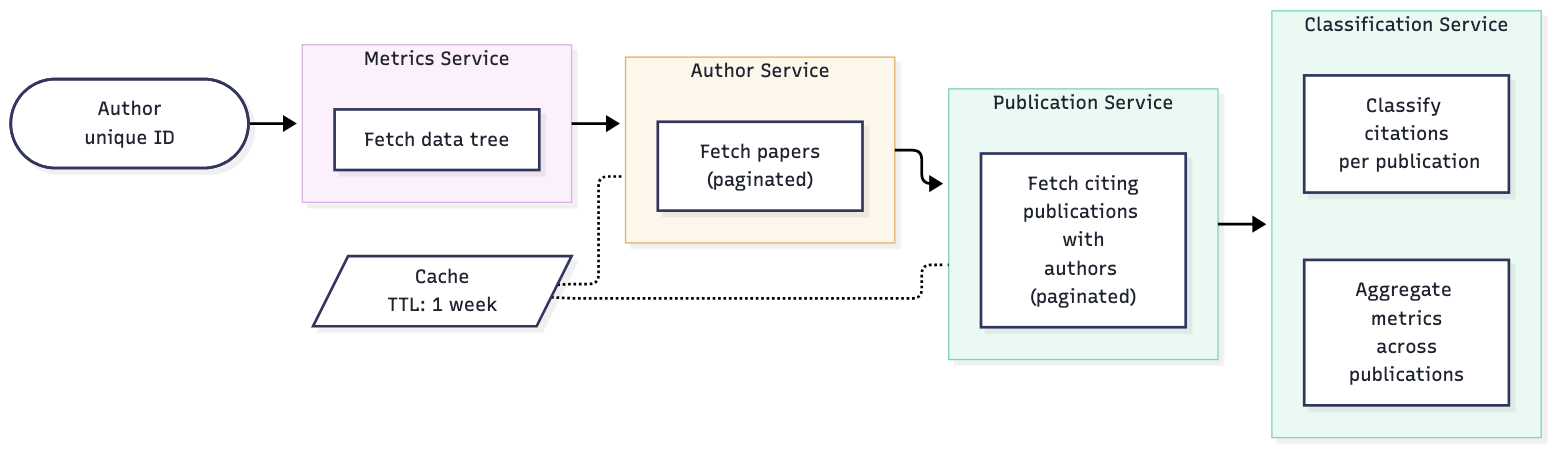
\includegraphics[height=.48\textheight]{fig-classification-flowchart-diagram}
  \vspace{1ex}
  \begin{itemize}
    \item Runs as a background job; the user follows the progress
    \item Requests are queued per provider, within its rate limit
    \item Responses are cached; the graph is stored, so results can be reopened later
  \end{itemize}
\end{frame}

% 14
\begin{frame}{Finding the right author}
  \begin{columns}[c]
    \begin{column}{.42\textwidth}
      \begin{itemize}
        \item One search covers all providers, one tab each
        \item Many researchers share a name
        \item Affiliation and provider identifier per profile
        \item \uicontrol{switch-show-papers-all} lists publications to recognize the author
      \end{itemize}
    \end{column}
    \begin{column}{.56\textwidth}
      \centering
      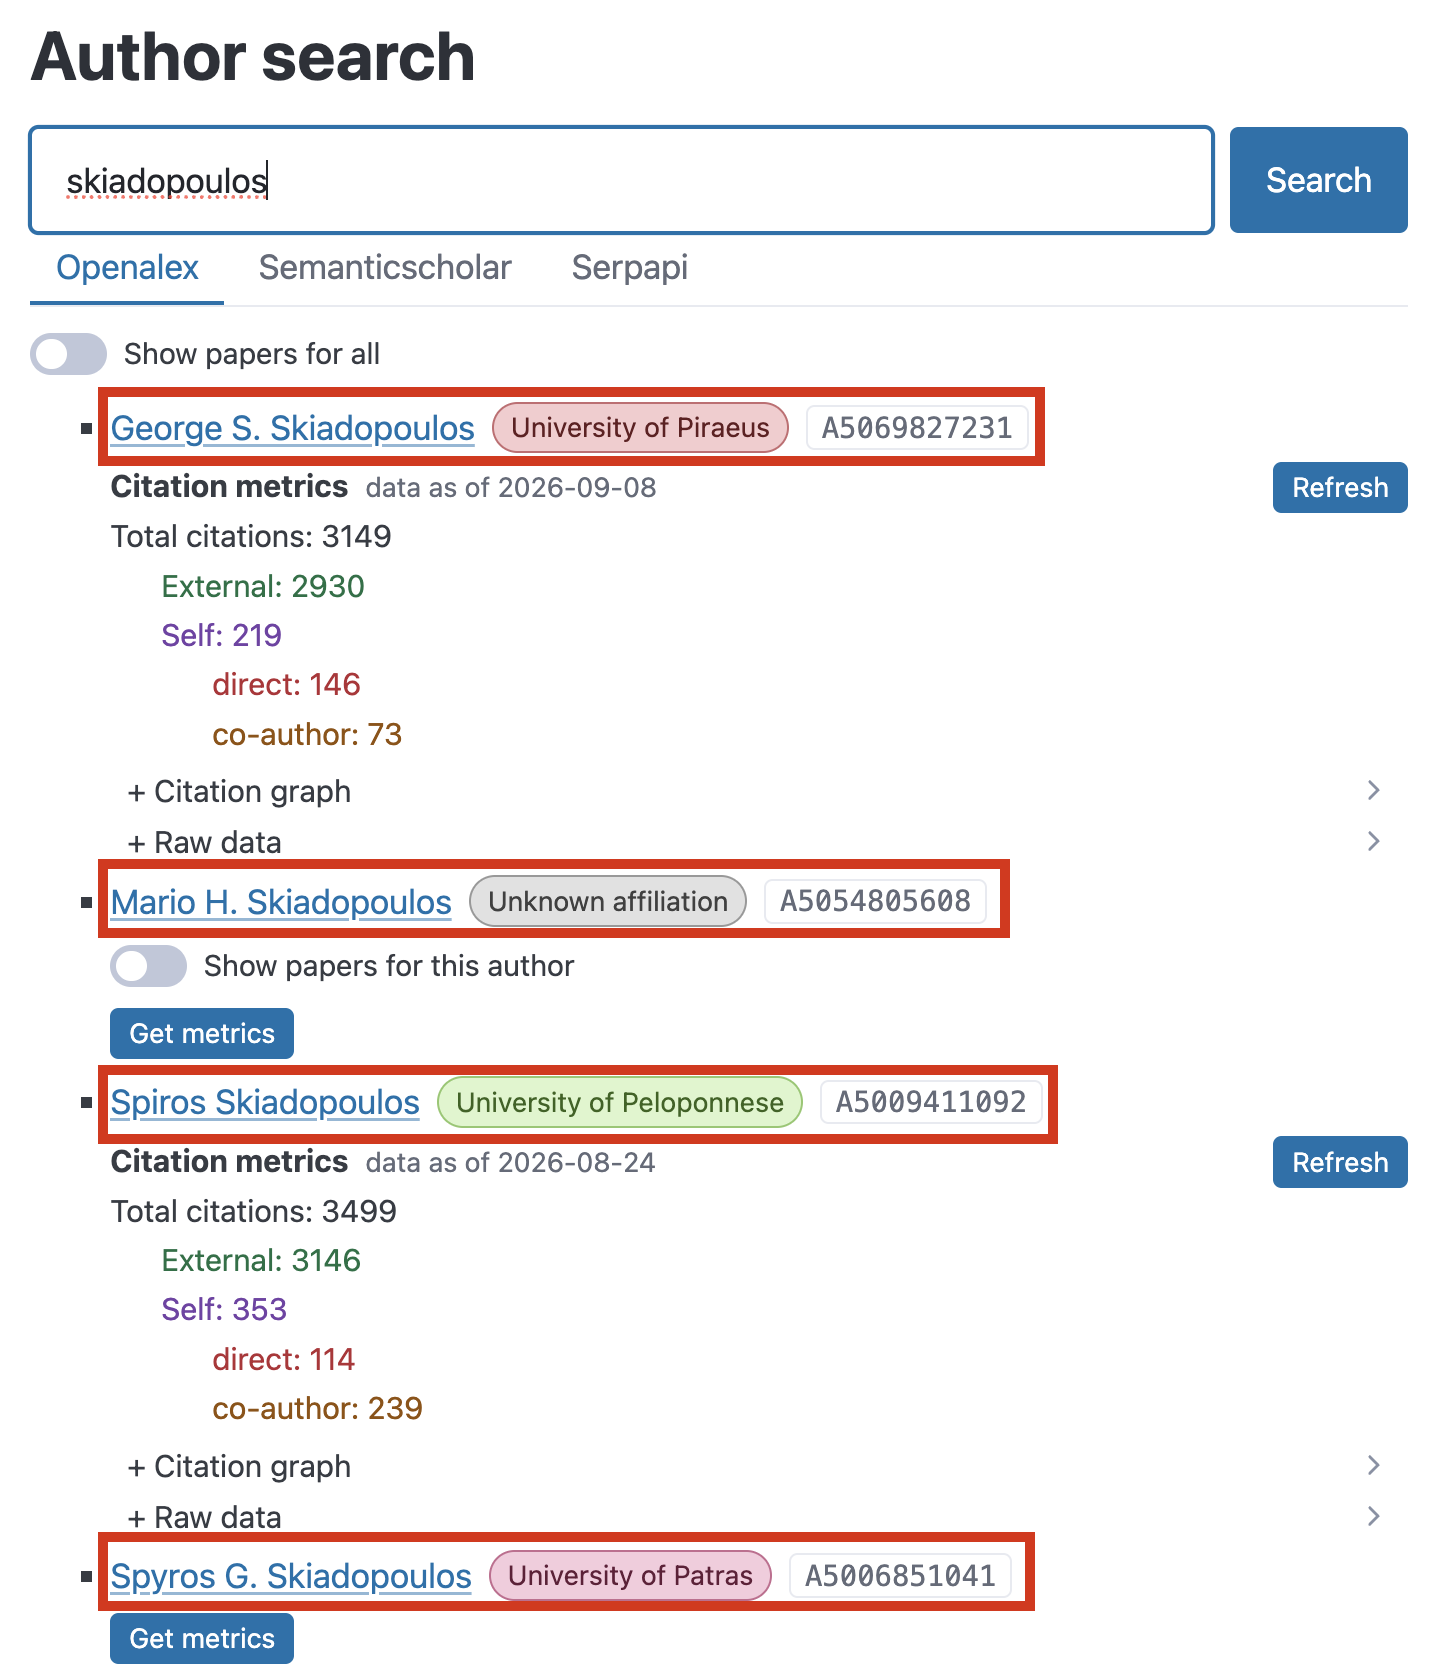
\includegraphics[height=.78\textheight]{ui/search-res-1}
    \end{column}
  \end{columns}
\end{frame}

% 15
\begin{frame}{Citation metrics}
  \begin{columns}[c]
    \begin{column}{.42\textwidth}
      \begin{itemize}
        \item \uicontrol{btn-get-metrics} starts the collection
        \item Progress: requests done, queued and failed
        \item Result: total, external, direct and co-author self-citations
        \item Stored results can be refreshed
      \end{itemize}
    \end{column}
    \begin{column}{.56\textwidth}
      \centering
      
\includegraphics[width=\textwidth]{ui/search-form-2}\\[2ex]
      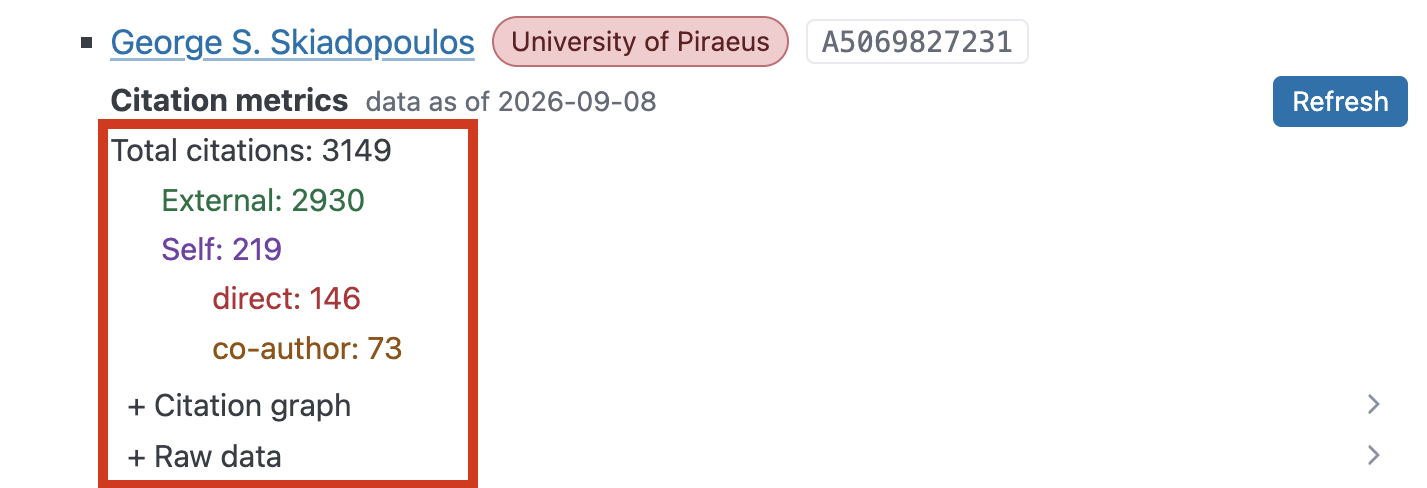
\includegraphics[width=\textwidth]{ui/search-res-7}
    \end{column}
  \end{columns}
\end{frame}

% 16
\begin{frame}{Citation graph}
  \begin{columns}[c]
    \begin{column}{.36\textwidth}
      \begin{itemize}
        \item Diamond: selected author
        \item Triangles: their papers
        \item Circles: citing papers, colored by classification
        \item Legend acts as a filter
        \item Zoom, pan, hover for details
      \end{itemize}
    \end{column}
    \begin{column}{.62\textwidth}
      \centering
      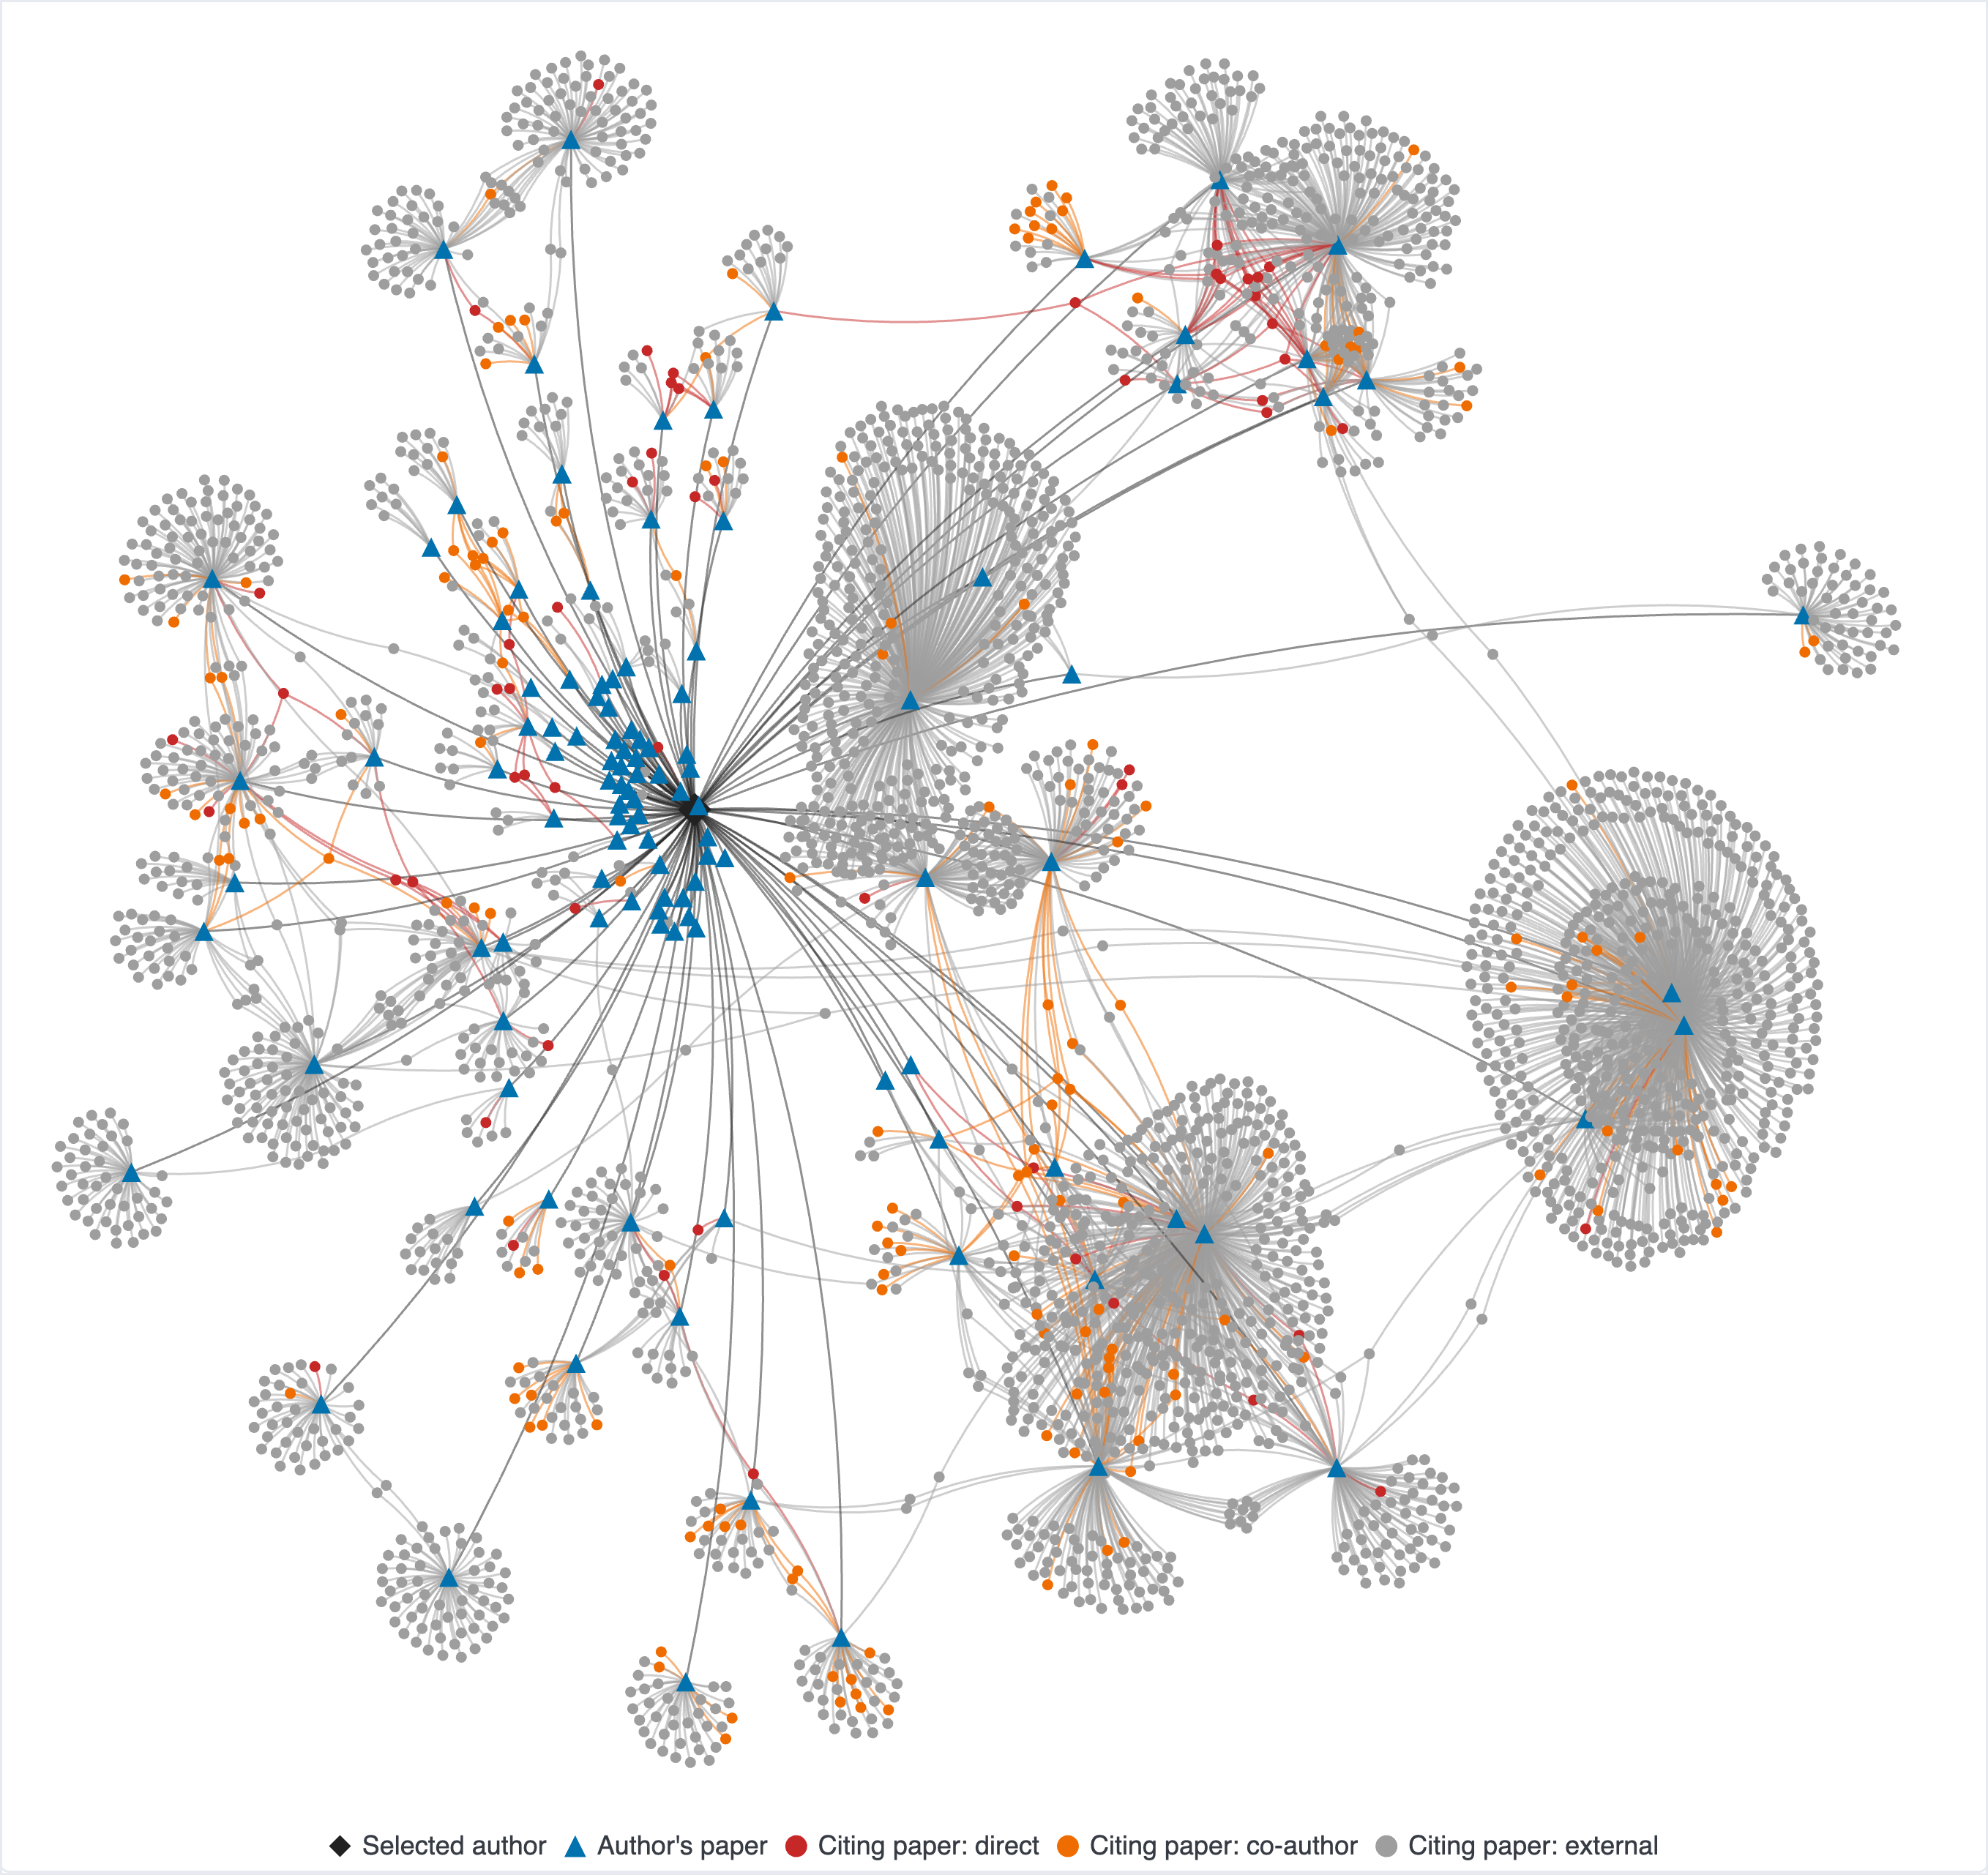
\includegraphics[height=.85\textheight]{ui/author-details-2}
    \end{column}
  \end{columns}
\end{frame}

% 17
\begin{frame}{Validating the classification}
  \begin{itemize}
    \item One author (Spiros Skiadopoulos), one provider (OpenAlex)
    \item Independent count with SQL queries over the stored graph
  \end{itemize}
  \vspace{1ex}
  \centering
  \begin{tabular}{rrrr}
    \toprule
    Total & Direct & Co-author & External \\
    \midrule
    3584 & 115 & 243 & 3226 \\
    \bottomrule
  \end{tabular}
  \vspace{1ex}

  $115 + 243 + 3226 = 3584$, matching the counts calculated by the system
\end{frame}

% 18
\begin{frame}{Comparing the sources}
  \begin{columns}[c]
    \begin{column}{.58\textwidth}
      \scriptsize
      \begin{tabular}{lrrrr}
        \toprule
        Provider & Papers & Citations & Self & External \\
        \midrule
        OpenAlex & 117 & 3584 & 10.0\% & 90.0\% \\
        Semantic Scholar & 187 & 4093 & 8.6\% & 91.4\% \\
        Google Scholar & 157 & 5458 & 1.4\% & 98.6\% \\
        \bottomrule
      \end{tabular}
      \normalsize
      \begin{itemize}
        \item Only 71 of 236 titles in all three sources
        \item OpenAlex and Semantic Scholar agree on 99\% of shared citations
        \item Google Scholar: names as text, self-citations largely missed
      \end{itemize}
    \end{column}
    \begin{column}{.4\textwidth}
      \centering
      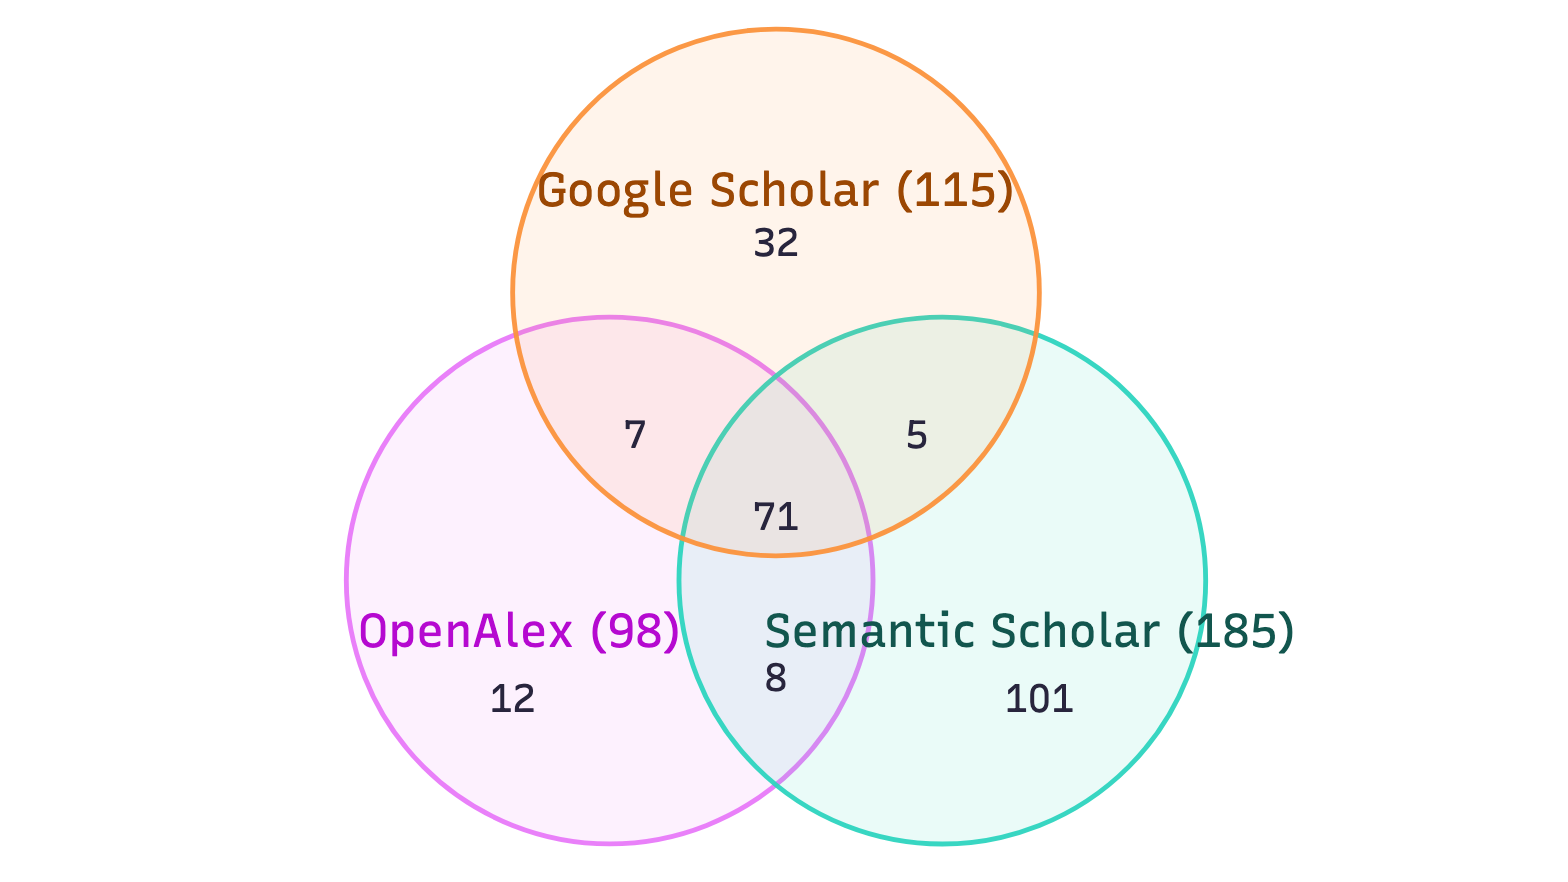
\includegraphics[width=\textwidth]{fig-provider-distribution-diagram}
    \end{column}
  \end{columns}
\end{frame}

% 19
\begin{frame}{Conclusions}
  \begin{itemize}
    \item The state of the available data sources remains an open problem
      \begin{itemize}
        \item OpenAlex was the most dependable source
        \item the others are limited in access, completeness and data quality
      \end{itemize}
    \item There is no consensus on how to classify citations
      \begin{itemize}
        \item author contributions are ambiguous
        \item our classification keeps the different views apart
      \end{itemize}
    \item Citation analysis is graph analysis: build the graph, then traverse it
    \item Current technologies made a single-user interactive prototype straightforward
  \end{itemize}
\end{frame}

% 20
\begin{frame}{Future work}
  \begin{itemize}
    \item \alert{Combining the data sources}
      \begin{itemize}
        \item match authors and papers across sources
        \item no universally adopted identifiers: match similar names and titles
      \end{itemize}
    \item \alert{Detecting circular citations}
      \begin{itemize}
        \item $A_1 \rightarrow A_2 \rightarrow A_3 \rightarrow A_4 \rightarrow A_1$: no single citation is a self-citation
        \item requires extending the graph beyond a single level
      \end{itemize}
  \end{itemize}
  \vfill
  \centering
  \Large Thank you \textendash{} questions?
\end{frame}

% Backup slides for technical questions; not counted in the 20 main slides.
\appendix

\begin{frame}[noframenumbering]{Backup: backend layers}
  \begin{description}
    \item[Controllers] validate requests and call the services; one class per use case
    \item[Services] the only place with business logic: authors, publications, classification, citation graph, jobs, metrics
    \item[Connectors] one per provider, the same interface (\texttt{searchAuthors}, \texttt{getAuthorPublications}, \texttt{getCitations}); hide pagination, authentication, response formats
    \item[Repositories] one per table, queries through the Drizzle ORM; schema and migrations in code
  \end{description}
  \vspace{1ex}
  Dependencies are injected, so every unit can be tested in isolation.
\end{frame}

\begin{frame}[noframenumbering]{Backup: database}
  \centering
  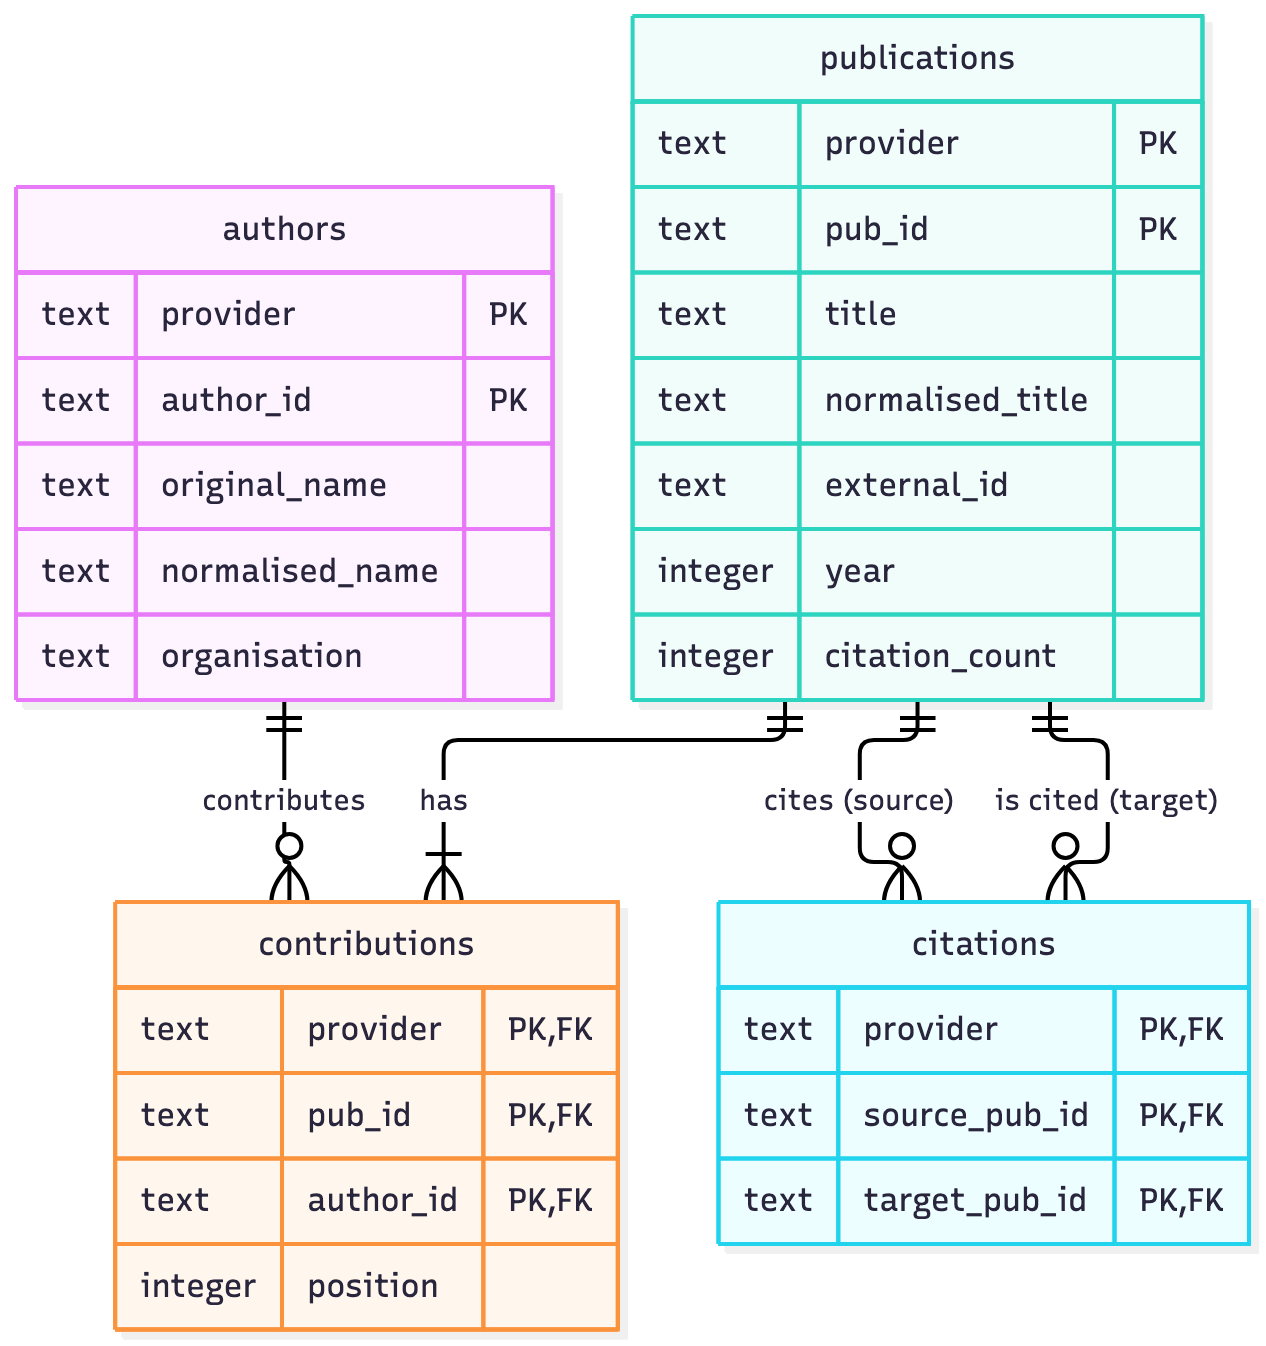
\includegraphics[height=.66\textheight]{fig-database-er-diagram}
  \hspace{2em}
  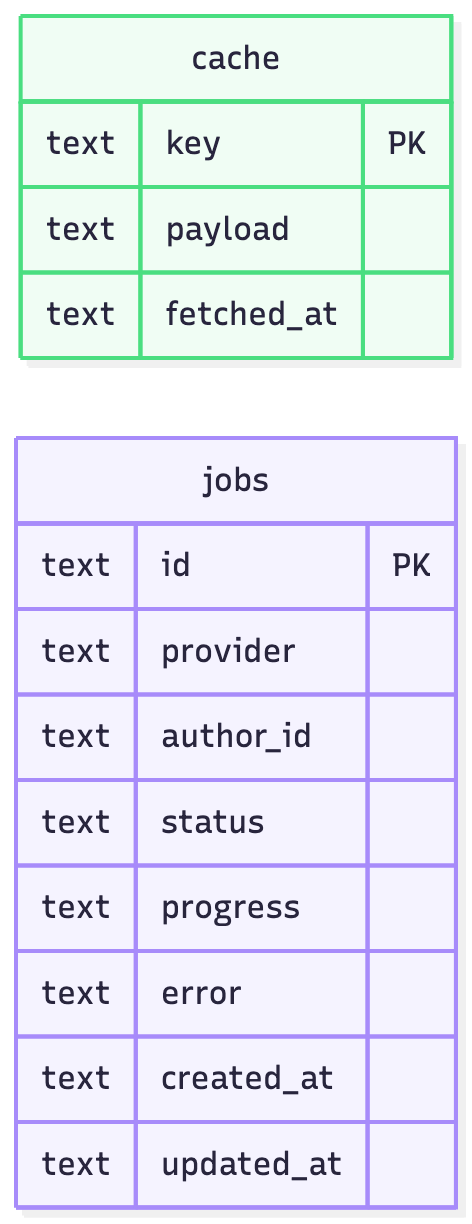
\includegraphics[height=.66\textheight]{fig-database-aux-er-diagram}\\[1ex]
  \small Composite keys include the provider; normalized names and titles are stored alongside the originals.
\end{frame}

\begin{frame}[noframenumbering]{Backup: caching and rate limits}
  \centering
  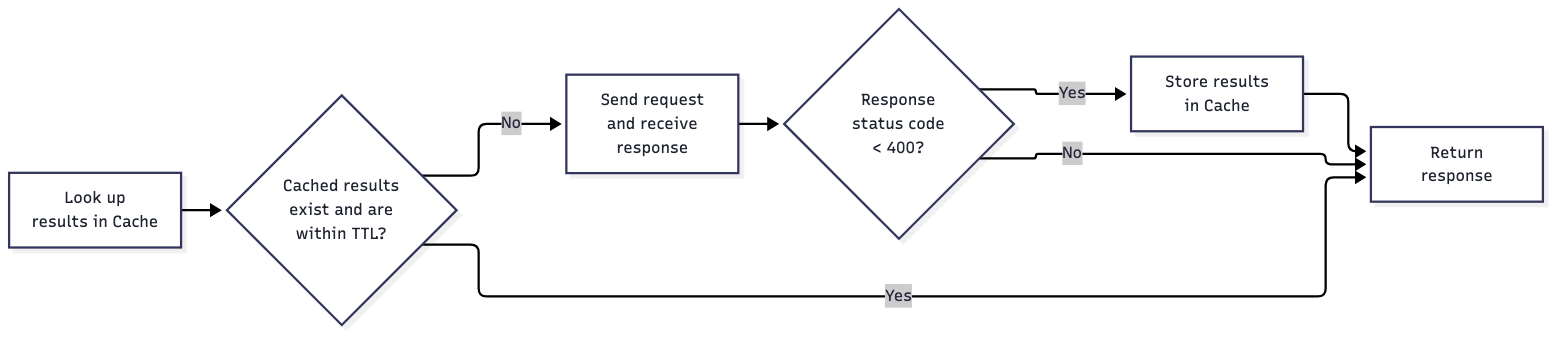
\includegraphics[height=.36\textheight]{fig-cache-flowchart-diagram}
  \vspace{1ex}
  \begin{itemize}
    \item Shared HTTP client; the cache key is the request URL with sorted query parameters
    \item Per-provider queues keep requests within the rate limit
    \item An author with $n$ publications needs at least $n$ citation requests
    \item No retention policy yet: the database can grow indefinitely
  \end{itemize}
\end{frame}

\begin{frame}[noframenumbering]{Backup: classification in SQL}
  \footnotesize
  \begin{itemize}
    \item \texttt{author\_citations}: citations whose target is a publication of the author
    \item \texttt{direct\_citations}: the source is also a publication of the author
    \item \texttt{coauthor\_citations}: the rest, where the source and target share any author
    \item \texttt{external\_citations}: the rest, with no shared author
  \end{itemize}
  \vspace{1ex}
  The three subsets are disjoint and add up to the total, which is how the system output was checked.
\end{frame}

\begin{frame}[noframenumbering]{Backup: testing}
  \begin{itemize}
    \item Backend unit tests with Jest, one suite per component
    \item No real databases, clock or network: every dependency is mocked
    \item Mocks reproduce provider errors, malformed data and empty results
    \item Nested scenarios: \texttt{describe} blocks refine the case, each \texttt{it} asserts one outcome
    \item GitHub Actions runs the tests on every push and blocks failing builds
  \end{itemize}
\end{frame}

\end{document}
